% Options for packages loaded elsewhere
\PassOptionsToPackage{unicode}{hyperref}
\PassOptionsToPackage{hyphens}{url}
%
\documentclass[
]{article}
\usepackage{lmodern}
\usepackage{amssymb,amsmath}
\usepackage{ifxetex,ifluatex}
\ifnum 0\ifxetex 1\fi\ifluatex 1\fi=0 % if pdftex
  \usepackage[T1]{fontenc}
  \usepackage[utf8]{inputenc}
  \usepackage{textcomp} % provide euro and other symbols
\else % if luatex or xetex
  \usepackage{unicode-math}
  \defaultfontfeatures{Scale=MatchLowercase}
  \defaultfontfeatures[\rmfamily]{Ligatures=TeX,Scale=1}
\fi
% Use upquote if available, for straight quotes in verbatim environments
\IfFileExists{upquote.sty}{\usepackage{upquote}}{}
\IfFileExists{microtype.sty}{% use microtype if available
  \usepackage[]{microtype}
  \UseMicrotypeSet[protrusion]{basicmath} % disable protrusion for tt fonts
}{}
\makeatletter
\@ifundefined{KOMAClassName}{% if non-KOMA class
  \IfFileExists{parskip.sty}{%
    \usepackage{parskip}
  }{% else
    \setlength{\parindent}{0pt}
    \setlength{\parskip}{6pt plus 2pt minus 1pt}}
}{% if KOMA class
  \KOMAoptions{parskip=half}}
\makeatother
\usepackage{xcolor}
\IfFileExists{xurl.sty}{\usepackage{xurl}}{} % add URL line breaks if available
\IfFileExists{bookmark.sty}{\usepackage{bookmark}}{\usepackage{hyperref}}
\hypersetup{
  pdftitle={Assessment 1 - Linear Regression},
  hidelinks,
  pdfcreator={LaTeX via pandoc}}
\urlstyle{same} % disable monospaced font for URLs
\usepackage[margin=1in]{geometry}
\usepackage{color}
\usepackage{fancyvrb}
\newcommand{\VerbBar}{|}
\newcommand{\VERB}{\Verb[commandchars=\\\{\}]}
\DefineVerbatimEnvironment{Highlighting}{Verbatim}{commandchars=\\\{\}}
% Add ',fontsize=\small' for more characters per line
\usepackage{framed}
\definecolor{shadecolor}{RGB}{248,248,248}
\newenvironment{Shaded}{\begin{snugshade}}{\end{snugshade}}
\newcommand{\AlertTok}[1]{\textcolor[rgb]{0.94,0.16,0.16}{#1}}
\newcommand{\AnnotationTok}[1]{\textcolor[rgb]{0.56,0.35,0.01}{\textbf{\textit{#1}}}}
\newcommand{\AttributeTok}[1]{\textcolor[rgb]{0.77,0.63,0.00}{#1}}
\newcommand{\BaseNTok}[1]{\textcolor[rgb]{0.00,0.00,0.81}{#1}}
\newcommand{\BuiltInTok}[1]{#1}
\newcommand{\CharTok}[1]{\textcolor[rgb]{0.31,0.60,0.02}{#1}}
\newcommand{\CommentTok}[1]{\textcolor[rgb]{0.56,0.35,0.01}{\textit{#1}}}
\newcommand{\CommentVarTok}[1]{\textcolor[rgb]{0.56,0.35,0.01}{\textbf{\textit{#1}}}}
\newcommand{\ConstantTok}[1]{\textcolor[rgb]{0.00,0.00,0.00}{#1}}
\newcommand{\ControlFlowTok}[1]{\textcolor[rgb]{0.13,0.29,0.53}{\textbf{#1}}}
\newcommand{\DataTypeTok}[1]{\textcolor[rgb]{0.13,0.29,0.53}{#1}}
\newcommand{\DecValTok}[1]{\textcolor[rgb]{0.00,0.00,0.81}{#1}}
\newcommand{\DocumentationTok}[1]{\textcolor[rgb]{0.56,0.35,0.01}{\textbf{\textit{#1}}}}
\newcommand{\ErrorTok}[1]{\textcolor[rgb]{0.64,0.00,0.00}{\textbf{#1}}}
\newcommand{\ExtensionTok}[1]{#1}
\newcommand{\FloatTok}[1]{\textcolor[rgb]{0.00,0.00,0.81}{#1}}
\newcommand{\FunctionTok}[1]{\textcolor[rgb]{0.00,0.00,0.00}{#1}}
\newcommand{\ImportTok}[1]{#1}
\newcommand{\InformationTok}[1]{\textcolor[rgb]{0.56,0.35,0.01}{\textbf{\textit{#1}}}}
\newcommand{\KeywordTok}[1]{\textcolor[rgb]{0.13,0.29,0.53}{\textbf{#1}}}
\newcommand{\NormalTok}[1]{#1}
\newcommand{\OperatorTok}[1]{\textcolor[rgb]{0.81,0.36,0.00}{\textbf{#1}}}
\newcommand{\OtherTok}[1]{\textcolor[rgb]{0.56,0.35,0.01}{#1}}
\newcommand{\PreprocessorTok}[1]{\textcolor[rgb]{0.56,0.35,0.01}{\textit{#1}}}
\newcommand{\RegionMarkerTok}[1]{#1}
\newcommand{\SpecialCharTok}[1]{\textcolor[rgb]{0.00,0.00,0.00}{#1}}
\newcommand{\SpecialStringTok}[1]{\textcolor[rgb]{0.31,0.60,0.02}{#1}}
\newcommand{\StringTok}[1]{\textcolor[rgb]{0.31,0.60,0.02}{#1}}
\newcommand{\VariableTok}[1]{\textcolor[rgb]{0.00,0.00,0.00}{#1}}
\newcommand{\VerbatimStringTok}[1]{\textcolor[rgb]{0.31,0.60,0.02}{#1}}
\newcommand{\WarningTok}[1]{\textcolor[rgb]{0.56,0.35,0.01}{\textbf{\textit{#1}}}}
\usepackage{graphicx,grffile}
\makeatletter
\def\maxwidth{\ifdim\Gin@nat@width>\linewidth\linewidth\else\Gin@nat@width\fi}
\def\maxheight{\ifdim\Gin@nat@height>\textheight\textheight\else\Gin@nat@height\fi}
\makeatother
% Scale images if necessary, so that they will not overflow the page
% margins by default, and it is still possible to overwrite the defaults
% using explicit options in \includegraphics[width, height, ...]{}
\setkeys{Gin}{width=\maxwidth,height=\maxheight,keepaspectratio}
% Set default figure placement to htbp
\makeatletter
\def\fps@figure{htbp}
\makeatother
\setlength{\emergencystretch}{3em} % prevent overfull lines
\providecommand{\tightlist}{%
  \setlength{\itemsep}{0pt}\setlength{\parskip}{0pt}}
\setcounter{secnumdepth}{-\maxdimen} % remove section numbering

\title{Assessment 1 - Linear Regression}
\author{}
\date{\vspace{-2.5em}}

\begin{document}
\maketitle

In this assessment, you need to answer all the questions about KNN,
Linear Regression, Regularization, Logistic Regression, K-fold
cross-validation, and other concepts covered in Module 1-3. R studio is
recommended to use to complete your assessment. All codes need comments
to help markers to understand your idea. If no comment is given, you may
have a 10\% redundancy on your mark. Please refer to weekly activities
as examples for how to write comments. After you have answered all the
questions, please knit your R notebook file to HTML or PDF format.
Submit both .rmd file and .html or .pdf file to assessment 1 dropbox via
the link on the Assessment page. You can compress your files into a zip
file for submission. The total mark of this assessment is 100, which
worths 30\% of your final result.

hint: Please review all reading materials in Module 1-3 carefully,
especially the activities.

\textbf{Question 1 - KNN (20 marks)}

\emph{In this question you are required to implement a KNN classifier to
predict the class of iris plants. The well-known iris dataset is used in
this question. Detailed description of this data set can be found at
\url{https://archive.ics.uci.edu/ml/datasets/iris}.}

\emph{Specifically, you need to:}

In this question, it is expected that the iris dataset will be split
into training and test data sets using a ratio of 7:3 and then run
through a KNN classifier in order to predict the class of iris plants.
Firstly, it is useful to visualise the data in order to get a general
understanding of iris dataset. Below is a scatterplot comparing the
variables \emph{Sepal.width} and \emph{Sepal.length} using the species
to catagorise them.

\begin{Shaded}
\begin{Highlighting}[]
\CommentTok{#load in iris data from datasets package}
\KeywordTok{library}\NormalTok{(datasets)}
\KeywordTok{data}\NormalTok{(iris)}

\CommentTok{#create scatterplot to illistrate petal measurement and visualise the data }
\KeywordTok{ggplot}\NormalTok{(}\DataTypeTok{data =}\NormalTok{ iris, }\KeywordTok{aes}\NormalTok{(}\DataTypeTok{x =}\NormalTok{ Sepal.Length, }\DataTypeTok{y =}\NormalTok{ Sepal.Width, }\DataTypeTok{color =}\NormalTok{ Species)) }\OperatorTok{+}\StringTok{ }
\StringTok{    }\KeywordTok{geom_point}\NormalTok{() }\OperatorTok{+}\StringTok{ }\KeywordTok{geom_rug}\NormalTok{()}\OperatorTok{+}\StringTok{ }\KeywordTok{theme_minimal}\NormalTok{() }\OperatorTok{+}\StringTok{ }\KeywordTok{ggtitle}\NormalTok{(}\StringTok{"Petal Measurements"}\NormalTok{)}
\end{Highlighting}
\end{Shaded}

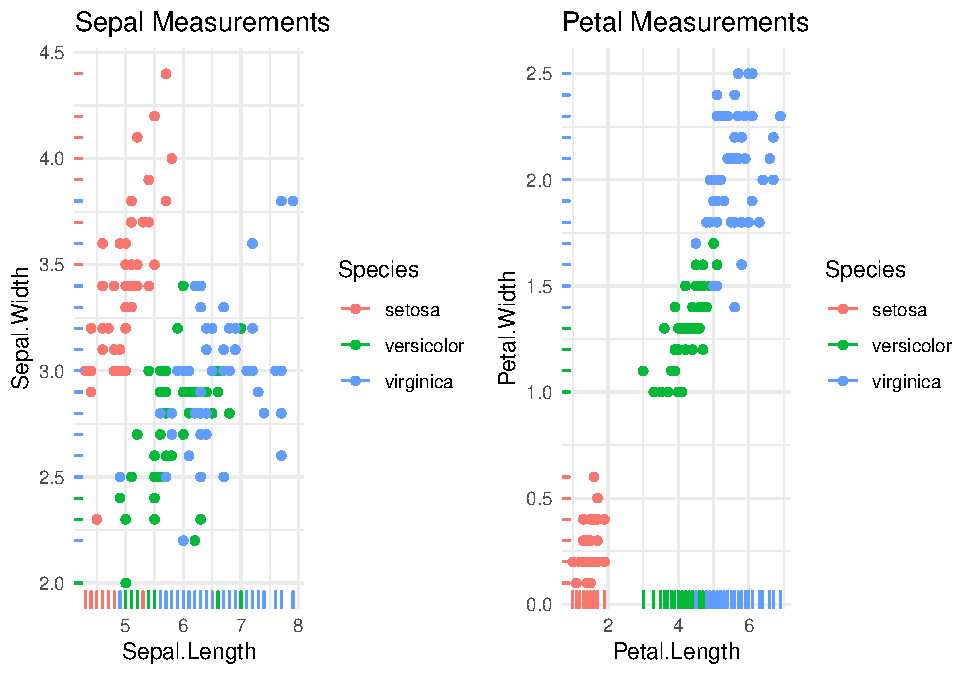
\includegraphics{assessment-1_files/figure-latex/unnamed-chunk-1-1.pdf}

\begin{enumerate}
\def\labelenumi{\arabic{enumi}.}
\tightlist
\item
  Split the data set into a training and a test set with the ratio of
  7:3. (1 mark)
\end{enumerate}

\begin{Shaded}
\begin{Highlighting}[]
\CommentTok{### 1. split the dataset into a training and a test set with the ratio of}
\CommentTok{### 7:3}

\CommentTok{#set random seed}
\KeywordTok{set.seed}\NormalTok{(}\DecValTok{001}\NormalTok{)}


\CommentTok{#}
\end{Highlighting}
\end{Shaded}

\begin{enumerate}
\def\labelenumi{\arabic{enumi}.}
\setcounter{enumi}{1}
\item
  Implement a KNN classifier. (5 marks)
\item
  Investigate the impact of different K (from 1 to 6) values on the
  model performance (ACC) and the impact of different distance
  measurements (euclidean, manhattan, canberra, and minkowski) on the
  model performance (ACC). Visualize and discuss your findings. (14
  marks)
\end{enumerate}

\hypertarget{question-2---linear-regression-35-marks}{%
\subsection{Question 2 - Linear Regression (35
marks)}\label{question-2---linear-regression-35-marks}}

In this question you need to implement a linear regression model to
predict health care cost. The data set used in this question can be
found in `insurance.csv'. The data set has 7 features, which are
summarized as below.

\begin{itemize}
\tightlist
\item
  Age: insurance contractor age, years
\item
  Sex: insurance contractor gender, {[}female, male{]}
\item
  BMI: Body mass index, providing an understanding of body, weights that
  are relatively high or low relative to height, objective index of body
  weight (kg / m \^{} 2) using the ratio of height to weight, ideally
  18.5 to 24.9
\item
  Children: number of children covered by health insurance / Number of
  dependents
\item
  Smoker: smoking, {[}yes, no{]}
\item
  Region: the beneficiary's residential area in the US, {[}northeast,
  southeast, southwest, northwest{]}
\item
  Charges: Individual medical costs billed by health insurance, \$
  \#predicted value
\end{itemize}

Specifically, you need to:

\begin{enumerate}
\def\labelenumi{\arabic{enumi}.}
\tightlist
\item
  Perform data pre-processing, including removing invalid data and
  transfromatting the categorical features to numerical features. (4
  marks)
\item
  Split the data set into a training set and a test set, with ratio of
  7:3. (2 mark)
\item
  Implement a linear regression model and train the model with your
  training data. Visualize the parameter updating process, test error
  (RMSE) in each iteration, and cost convergence process. Please be
  advised that built-in models in any realeased R package, like glm, is
  not allowed to use in this question. You can choose your preferred
  learning rate and determine the best iteration number. (8 marks)
\item
  Evaluate your model by calculating the RMSE, and visualizing the
  residuals of test data. Please note that explanation of your residual
  plot is needed. (5 marks)
\item
  Does your model overfit? Which features do you think are not
  significant? Please justify your answers. For example, you can analyze
  the significance of a feature from correlation, variance, etc. (8
  marks)
\item
  Use the glmnet library to biult two linear regression models with
  Lasso and Ridge regularization, respectively. In comparison to your
  model, how well do these two models perform? Do the regularized models
  automatically filter out the less significant features? What are the
  differences of these two models? Please justify your answers. (8
  marks)
\end{enumerate}

\begin{Shaded}
\begin{Highlighting}[]
\NormalTok{data =}\StringTok{ }\KeywordTok{read.csv}\NormalTok{(}\StringTok{'insurance.csv'}\NormalTok{)}
\end{Highlighting}
\end{Shaded}

\begin{Shaded}
\begin{Highlighting}[]
\CommentTok{# start your answer here ...}
\end{Highlighting}
\end{Shaded}

\hypertarget{question-3---logistic-regression-45-marks}{%
\subsection{Question 3 - Logistic Regression (45
marks)}\label{question-3---logistic-regression-45-marks}}

In this question, you are required to implement a Logistic Regression
model to classify whether a person donated blood at a Blood Transfusion
Service Center in March 2007. Please read the sub-questions below
carefully for the deteailed instructions.

\begin{enumerate}
\def\labelenumi{\arabic{enumi}.}
\tightlist
\item
  Check out the Blood Transfusion Service Center Data Set at
  \url{https://archive.ics.uci.edu/ml/datasets/Blood+Transfusion+Service+Center}.
\item
  Perform data preprocessing to determine and remove invalid samples.
  Split the data into a training set and a test set with a ratio of 7:3.
  (2 marks)
\item
  Develop a Logistic Regression model that use batch gradient descent
  for optimization. Visualize the parameter updating process, test error
  (ACC) in each iteration, and the cost convergence process. Please note
  that you need to develop your model step-by-step, built-in models in
  any realeased R package, like glm, is not allowed to use in this
  question. (10 marks)
\item
  Invesitigate the influence of different learning rate to the training
  process and answer what happend if you apply a too small or a too
  large learning rate. (5 marks)
\item
  Expermently compare batch gradient descent and stochastic gradient
  descent and discuss your findings (e.g., convergence speed). Visualize
  the comparison in terms of updating process and the cost convergence
  process. (6 marks)
\item
  Develop a K-fold (K = 5) cross validation to evaluate your model in
  step 3. Please note that you need to write R codes to explicitly show
  how you perform the K-fold cross validation. Built-in validation
  methods are not allowed to use. Different metrics, e.g.~ACC, Recall,
  precision, etc, should be used to evaluate your model. (8 marks)
\item
  Use different values of K (from 5 to N, where N denotes the sample
  number) and summarize the corresponding changes of your model
  performances. Visualize and explain the changes. (6 marks)
\item
  How can you modify the cost function to prevent overfitting? Discuss
  the possibility of adding regularization term(s) and summarize the
  possible changes in the gradient descent process. (8 marks)
\end{enumerate}

\begin{Shaded}
\begin{Highlighting}[]
\CommentTok{# start your answer here ...}
\end{Highlighting}
\end{Shaded}

\end{document}
